%\documentclass[12pt]{report}
%\setlength{\parindent}{0mm}
%\setlength{\parskip}{14pt}
%\renewcommand{\baselinestretch}{2.0}
%\setlength{\topmargin}{0pt}
%\setlength{\headheight}{0pt}
%\setlength{\headsep}{0pt}
%\setlength{\footskip}{45pt}
%\setlength{\textwidth}{465pt}
%\setlength{\textheight}{660pt}
%\setlength{\oddsidemargin}{10pt}
%\newcommand{\RR}{\mathrm{I\!R\!}}
%\newcommand{\FF}{\mathrm{I\!F\!}}
%\newcommand{\dt}{\frac{\partial}{\partial t}}
%\newcommand{\dq}{\frac{\partial}{\partial q }}
%\newcommand{\dr}{\frac{\partial}{\partial p }}
%\newtheorem{defi}{Definition}[chapter]
%\newtheorem{theo}{Theorem}[chapter]

%\begin{document}

\chapter{Discretization of the Navier-Stokes Equations}

In this chapter, we discuss the finite-differencing scheme for the discretization of the Navier-Stokes equations as well as describe in detail Chorin's Projection Method for solving the resulting Poisson equation for pressure.

\section{Finite Difference Approximations}

\subsection{First Order Finite Difference Approximations}

In order to work efficiently with the series that follow, we introduce the concept of the Big-O notation.

\begin{defi}
Let $f(x)$ and $g(x)$ be two functions defined on a subset of real numbers. We say that $f(x)$ is \textbf{Big-O} of $g(x)$  if there exist positive real numbers $C$ and $x_{0}$ such that 
$$ \left|f(x)\right| \leq C\left|g(x)\right| \ \forall x > x_{0} $$

This can also be formulated to study the behavior of $f(x)$ near some real number $a$ as follows: Let $f(x)$ and $g(x)$ be two functions defined on a subset of real numbers. We say that $f(x)$ is \textbf{Big-O} of $g(x)$  if there exist positive real numbers $C$ and $\delta$ such that

$$ \left|f(x)\right| \leq C\left|g(x)\right| for \left|x-a\right| < \delta $$

\end{defi}

In order to perform the discretization of the governing equation for fluid motion, one must be able to approximate the continuous differential operator at a finite number of grid points. 
Consider a function $u(x,t)$ with $ x \in [0,L]$ and $ t \in [0,T]$. A discretization of the function $u$ is obtained by considering only
the values $u_{i}^{j}$ at a finite number of grid points $(x_{i},t_{j})$. Applying Taylor�s series expansion to $u(x_{i},t_{j}+\delta t)$ gives \begin{equation} u(x_{i},t_{j}+\delta t) = u(x_{i},t_{j}) + u_{t}(x_{i},t_{j}) \delta t + u_{tt}(x_{i},t_{j}) \frac{(\delta t)^2}{2} + u_{ttt}(x_{i},t_{j}) \frac{(\delta t)^3}{3!} + O((\delta t)^4) \end{equation} The following convention will be used in an effort to reduce the use of notation throughout this work. \begin{equation} u_{i}^{j} = u(x_{i},t_{j}) = u(i\delta x, j\delta t)\  i =0,1,\cdots ,m; \ j = 0,1,\cdots .n. \end{equation} Recasting the above equation with this in mind yields \begin{equation} \label{ffd}u_{i}^{j+1} = u_{i}^{j} + (u_{t})_{i}^{j} \delta t + (u_{tt})_{i}^{j} \frac{(\delta t)^2}{2} + (u_{ttt})_{i}^{j} \frac{(\delta t)^3}{3!} + O((\delta t)^4). \end{equation} Truncating this equation at the second order term and solving for $(u_{t})_{i}^{j}$ yields \begin{equation}  (u_{t})_{i}^{j} = \frac{u_{i}^{j+1} - u_{i}^{j}}{\delta t} + O(\delta t). \end{equation} Therefore \begin{equation} (u_{t})_{i}^{j} \approx \frac{u_{i}^{j+1} - u_{i}^{j}}{\delta t} \end{equation}
This equation is known as the two point forward finite difference approximation of $\displaystyle{\frac{\partial u}{\partial t}}.$ 

Applying Taylor�s series expansion to $u_{i}^{j-1}$ gives \begin{equation}\label{bfd} u_{i}^{j-1} = u_{i}^{j} - (u_{t})_{i}^{j} \delta t + (u_{tt})_{i}^{j} \frac{(\delta t)^2}{2} - (u_{ttt})_{i}^{j} \frac{(\delta t)^3}{3!} + O((\delta t)^4) \end{equation}

Truncating this equation at the second order term and solving for $(u_{t})_{i}^{j}$ yields \begin{equation}  (u_{t})_{i}^{j} = \frac{u_{i}^{j} - u_{i}^{j-1}}{\delta t} + O(\delta t). \end{equation} Therefore \begin{equation} (u_{t})_{i}^{j} \approx \frac{u_{i}^{j} - u_{i}^{j-1}}{\delta t} \end{equation}
 This equation is known as the two point backward finite difference approximation of $\displaystyle{\frac{\partial u}{\partial t}}.$

Doing the difference of equations (ffd) and (bfd) yield \begin{equation} u_{i}^{j+1} - u_{i}^{j-1} = 2(u_{t})_{i}^{j} \delta t + O((\delta t)^3). \end{equation} Solving for $(u_{t})_{i}^{j}$ yields \begin{equation} (u_{t})_{i}^{j} = \frac{u_{i}^{j+1} - u_{i}^{j-1}}{2\delta t} + O((\delta t)^2). \end{equation} Therefore \begin{equation} (u_{t})_{i}^{j} \approx \frac{u_{i}^{j+1} - u_{i}^{j-1}}{2\delta t} \end{equation} This equation is known as the two point central difference approximation of $\displaystyle{\frac{\partial u}{\partial t}}.$

The forward and backward finite difference approximation of $\displaystyle{\frac{\partial u}{\partial t}}.$ have an error of order $\delta t$ where as the central finite difference approximation of $\displaystyle{\frac{\partial u}{\partial t}}.$ has an error of order $(\delta t)^2$ which indicates that for most applications, the central finite difference approximation will yield more accurate results. All of the finite difference approximations for the spatial derivatives can be found in an analogous way to the difference approximations found for the time derivative.

\subsection{Higher Order Finite Difference Approximations}

Following a similar procedure to that used in the previous section, higher order finite difference approximations can be derived but only the second order central finite difference approximations will be investigated here.

To accomplish this, the Taylor Series Expansion is again found for $u_{i}^{j+1}$ and $u_{i}^{j-1}$. 

\begin{equation} u_{i}^{j-1} = u_{i}^{j} - (u_{t})_{i}^{j} \delta t + (u_{tt})_{i}^{j} \frac{(\delta t)^2}{2} - (u_{ttt})_{i}^{j} \frac{(\delta t)^3}{3!} + O((\delta t)^4) \end{equation}

\begin{equation} u_{i}^{j+1} = u_{i}^{j} + (u_{t})_{i}^{j} \delta t + (u_{tt})_{i}^{j} \frac{(\delta t)^2}{2} + (u_{ttt})_{i}^{j} \frac{(\delta t)^3}{3!} + O((\delta t)^4). \end{equation}

Taking the sum of these expansions yields
\begin{equation} u_{i}^{j-1} + u_{i}^{j+1} = 2u_{i}^{j} + (u_{tt})_{i}^{j}(\delta t)^2 + O((\delta t)^4) \end{equation}

Therefore, \begin{equation} (u_{tt})_{i}^{j} \approx \frac{u_{i}^{j-1}-2u_{i}^{j}+u_{i}^{j+1}}{(\delta t)^2} \end{equation}
 
This equation is known as the three point central difference approximation of $\displaystyle{\frac{\partial^2 u}{\partial t^2}}.$

The second order forward and backward finite difference approximations can be found by composing any of the first order approximations.

When dealing with Navier-Stokes equations, using a purely finite-difference discretization would lead to stability issues. We introduce the Donor-Cell discretization scheme in order to circumvent this stability issue. 

\section{The Donor-Cell Discretization Scheme}

We define the donor-cell discretization \cite{nsfd} of some convective term $\displaystyle{\frac{d(ku)}{dx}}$ by

\begin{equation}
\left[\frac{d(ku)}{dx}\right]_{i}^{dc} := \frac{k_{r}u_{r} - k_{l}u_{l}}{\delta x}
\end{equation}

where $u_r$ and $u_l$ are chosen based on the sign of $k_r$ and $k_l$, i.e.

$$ u_r := \left \{
\begin{array}{l r}
u_i & k_r > 0\\
u_{i+1} & k_r < 0
\end{array}
\right. \hspace{1in}
u_l := \left \{
\begin{array}{l r}
u_{i-1} & k_l > 0\\
u_{i} & k_l < 0
\end{array}
\right.$$

In order to avoid these case distinction, the donor-cell discretization can written as

\begin{equation}
\left[\frac{d(ku)}{dx}\right]_{i}^{dc} := \frac{1}{2\delta x}\left(k_{r}(u_{i} + u_{i+1}) - k_{l} (u_{i-1} + u_{i}) + \left|k_{r}\right|(u_{i} - u_{i+1}) - \left|k_{l}\right|(u_{i-1} - u_{i})\right)
\end{equation}

The need for this scheme will be explained in the sections covering the discretization of the Navier-Stokes equations.

\section{Discretization of the Heat Equation}

In this subsection, we introduce the finite difference approximation of the one-dimensional heat equation without sources on a finite interval $0<x<L$. Handling of the initial and boundary conditions will be ignored here and will be dealt with in detail for the Navier-Stokes Equations. The Heat Equation as specified is given by

\begin{eqnarray*}
\left \{
\begin{array}{l r}
\displaystyle{\frac{\partial u}{\partial t} = k\frac{\partial^2 u}{\partial x^2}}\\
 u(0,t)=0 & \\
u(L,t)=0 & \\
u(x,0)=f(x) & 
\end{array}
\right. 
\end{eqnarray*}

In order to discretize this equation, we replace the time derivative with its forward finite difference approximation and the space derivative with its central finite difference approximation yielding \begin{equation} \frac{u_{i}^{j+1} - u_{i}^{j}}{\Delta t} = k\frac{u_{i-1}^{j} -2u_{i}^{j} + u_{i+1}^{j}}{(\Delta x)^2}. \end{equation} The forward finite difference approximation was used for the time derivative because of the initial condition supplied and the central finite difference approximation was used for the space derivative because of the boundary conditions supplied. Since the truncated terms go to zero as $\Delta t$ and $\Delta x$ go to zero, the numerical approximate is said to be  \textbf{consistent} with the given PDE in its continuous form. The analysis for Navier-Stokes equations are now investigated.

\section{Discretization of the Spatial Derivative}

We use a staggered grid in order to discretize the Navier-Stokes Equations \cite{nsfd}. In this approach, the horizontal velocities $u$ are located at the midpoint of the vertical cell edges, the vertical velocities $v$ are located at the midpoint of the horizontal cell edges, and the pressure $p$ is located at the cell centers. Using the staggered grid approach eliminates the pressure oscillations that would occur with a grid in which $u$,$v$,and $p$ are all located at the same grid point.
\begin{figure}
\begin{center}
\caption{Staggered Grid}
\label{sg}
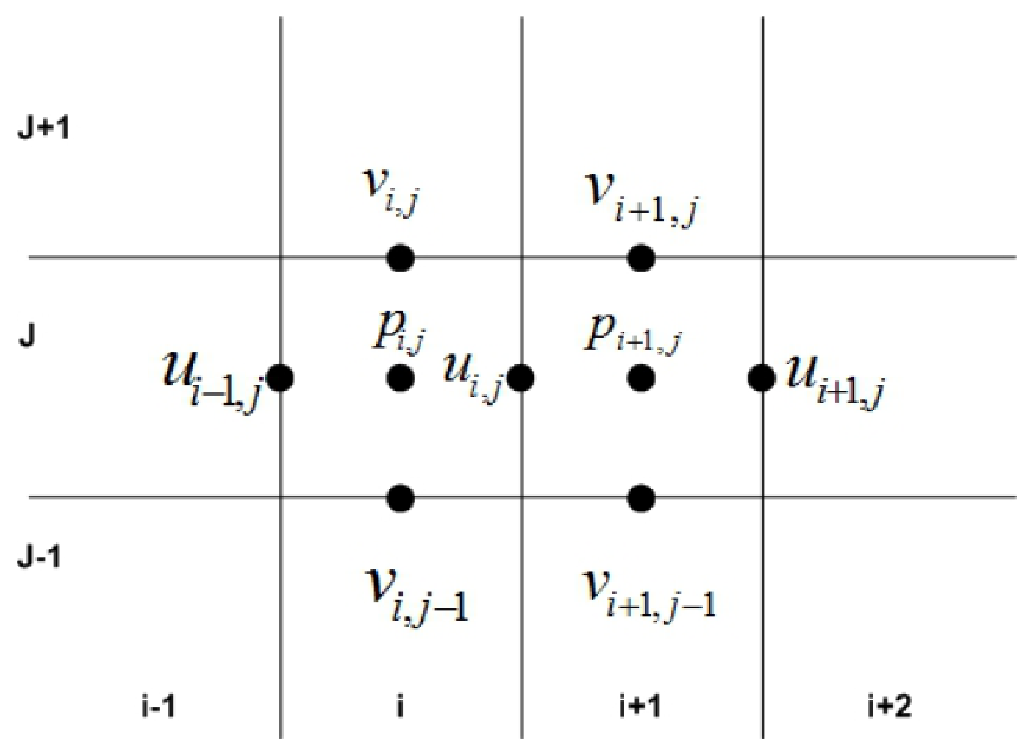
\includegraphics[scale = .5]{staggered_grid_marvin.eps}
\end{center}
\end{figure}
In order to discretize the continuity equation, we replace the spatial derivatives $\displaystyle{\frac{\partial u}{\partial x}}$ and $\displaystyle{\frac{\partial v}{\partial y}}$ by centered differences with half the mesh width. That is, 

\begin{equation}
\left[\frac{\partial u}{\partial x}\right]_{i}^{j} := \frac{u_{i}^{j} - u_{i-1}^{j}}{\delta x} \hspace{1in} \left[\frac{\partial v}{\partial y}\right]_{i}^{j} := \frac{v_{i}^{j} - v_{i}^{j-1}}{\delta y}
\end{equation}

The terms $\displaystyle{\frac{\partial^2 u}{\partial x^2}}$, $\displaystyle{\frac{\partial^2 u}{\partial y^2}}$,$\displaystyle{\frac{\partial^2 v}{\partial x^2}}$, and $\displaystyle{\frac{\partial^2 v}{\partial y^2}}$ in the momentum equation are replaced with the second order centered difference approximations as discussed earlier in the chapter. These terms form the so called diffusive terms of the momentum equations. The remaining terms present small complications due to the form of the grid spacing that was chosen. For the terms, $\displaystyle{\frac{\partial uv}{\partial y}}$ and $\displaystyle{\frac{\partial u^2}{\partial x}}$ we use the averages of \textbf{u},\textbf{v} and \textbf{u} respectively to obtain suitable values of the product lying in the two vertical directions. 
That is,

\begin{equation}
\left[\frac{\partial (uv)}{\partial y}\right]_{i}^{j} := \frac{1}{\delta y}\left(\frac{(v_{i}^{j} + v_{i+1}^{j})}{2} \frac{(u_{i}^{j} + u_{i}^{j+1})}{2} - \frac{(v_{i}^{j-1} + v_{i+1}^{j-1})}{2} \frac{(u_{i}^{j-1} + u_{i}^{j})}{2}\right)
\end{equation}

and

\begin{equation}
\left[\frac{\partial (u^2)}{\partial x}\right]_{i}^{j} := \frac{1}{\delta x}\left(\left(\frac{u_{i}^{j} + u_{i+1}^{j}}{2}\right)^2 - \left(\frac{u_{i-1}^{j} + u_{i}^{j}}{2}\right)^2\right)
\end{equation}

The terms $\displaystyle{\frac{\partial (uv)}{\partial x}}$ and $\displaystyle{\frac{\partial (u^2)}{\partial x}}$ are treated in an analogous fashion. Since at high Reynolds numbers the convective terms in our equation become dominant and may present problems with stability, a blend of the central differences and the donor-cell discretization is used. This leads to the following discretization.

\begin{eqnarray*} \left[\frac{\partial (u^2)}{\partial x}\right]_{i}^{j} := \frac{1}{\delta x}\left(\left(\frac{u_{i}^{j} + u_{i+1}^{j}}{2}\right)^2 - \left(\frac{u_{i-1}^{j} + u_{i}^{j}}{2}\right)^2\right)& &
& & + \gamma \frac{1}{\delta x} \left(\frac{\left|u_{i}^{j} + u_{i+1}^{j}\right|}{2}\frac{(u_{i}^{j} - u_{i+1}^{j})}{2} - \frac{\left|u_{i-1}^{j} + u_{i}^{j}\right|}{2}\frac{(u_{i-1}^{j} - u_{i}^{j})}{2}\right) \end{eqnarray*}

\begin{eqnarray*} \left[\frac{\partial (uv)}{\partial y}\right]_{i}^{j} := \frac{1}{\delta y}\left(\frac{(v_{i}^{j} + v_{i+1}^{j})}{2} \frac{(u_{i}^{j} + u_{i}^{j+1})}{2} - \frac{(v_{i}^{j-1} + v_{i+1}^{j-1})}{2} \frac{(u_{i}^{j-1} + u_{i}^{j})}{2}\right)& &
& & + \gamma \frac{1}{\delta y} \left(\frac{\left|v_{i}^{j} + v_{i+1}^{j}\right|}{2}\frac{(u_{i}^{j} - u_{i}^{j+1})}{2} - \frac{\left|v_{i}^{j-1} + v_{i+1}^{j-1}\right|}{2}\frac{(u_{i}^{j-1} - u_{i}^{j})}{2}\right) \end{eqnarray*}

$$ \left[\frac{\partial^2 u}{\partial x^2}\right]_{i}^{j} :=  \frac{u_{i+1}^{j} - 2u_{i}^{j} + u_{i-1}^{j}}{(\delta x)^2} $$

$$ \left[\frac{\partial^2 u}{\partial y^2}\right]_{i}^{j} :=  \frac{u_{i}^{j+1} - 2u_{i}^{j} + u_{i}^{j-1}}{(\delta y)^2} $$

$$ \left[\frac{\partial p}{\partial x}\right]_{i}^{j} :=  \frac{p_{i+1}^{j} - p_{i}^{j} }{(\delta x)} $$


\begin{eqnarray*} \left[\frac{\partial (v^2)}{\partial y}\right]_{i}^{j} := \frac{1}{\delta y}\left(\left(\frac{v_{i}^{j} + v_{i}^{j+1}}{2}\right)^2 - \left(\frac{v_{i}^{j-1} + v_{i}^{j}}{2}\right)^2\right)& &
& & + \gamma \frac{1}{\delta y} \left(\frac{\left|v_{i}^{j} + v_{i}^{j+1}\right|}{2}\frac{(v_{i}^{j} - u_{i}^{j+1})}{2} - \frac{\left|v_{i}^{j-1} + v_{i}^{j}\right|}{2}\frac{(v_{i}^{j-1} - v_{i}^{j})}{2}\right) \end{eqnarray*}

\begin{eqnarray*} \left[\frac{\partial (uv)}{\partial x}\right]_{i}^{j} := \frac{1}{\delta x}\left(\frac{(u_{i}^{j} + u_{i}^{j+1})}{2} \frac{(v_{i}^{j} + v_{i+1}^{j})}{2} - \frac{(u_{i-1}^{j} + u_{i-1}^{j+1})}{2} \frac{(v_{i-1}^{j} + v_{i}^{j})}{2}\right) & &
& & + \gamma \frac{1}{\delta x} \left(\frac{\left|u_{i}^{j} + u_{i}^{j+1}\right|}{2}\frac{(v_{i}^{j} - v_{i+1}^{j})}{2} - \frac{\left|u_{i-1}^{j} + u_{i-1}^{j+1}\right|}{2}\frac{(v_{i-1}^{j} - v_{i}^{j})}{2}\right) \end{eqnarray*}

$$ \left[\frac{\partial^2 v}{\partial x^2}\right]_{i}^{j} :=  \frac{v_{i+1}^{j} - 2v_{i}^{j} + v_{i-1}^{j}}{(\delta x)^2} $$

$$ \left[\frac{\partial^2 v}{\partial y^2}\right]_{i}^{j} :=  \frac{v_{i}^{j+1} - 2v_{i}^{j} + v_{i}^{j-1}}{(\delta y)^2} $$

$$ \left[\frac{\partial p}{\partial y}\right]_{i}^{j} :=  \frac{p_{i}^{j+1} - p_{i}^{j} }{(\delta y)} $$

The parameter $\gamma$ lies between 0 and 1 and should be chosen such that

$$ \displaystyle{\gamma \geq \max_{i,j} \left(\left|\frac{u_{i,j}\delta t}{\delta x}\right|,\left|\frac{v_{i,j}\delta t}{\delta y}\right|\right)} $$

Appropriately discretized boundary conditions must also be supplied depending on the nature of the problem being studied. 

\section{Discretization of the Time Derivative}

In order to discretize the time derivatives occurring in the momentum equations, first order finite differences are used \cite{nsfd}.  Doing this yields

\begin{equation}
\left[\frac{\partial u}{\partial t}\right]^{(n+1)} := \frac{u^{(n+1)} - u^{(n)}}{\delta t}, \hspace{1in} \left[\frac{\partial v}{\partial t}\right]^{(n+1)} := \frac{v^{(n+1)} - v^{(n)}}{\delta t}
\end{equation} 

\subsection{The Time-Stepping Algorithm}

The time-stepping algorithm begins by discretizing the time derivatives appearing in the momentum equation. As a result, we have

\begin{equation}
u^{(n+1)} = u^{(n)} + \delta t\left[\frac{1}{Re}\left(\frac{\partial^2 u}{\partial x^2} + \frac{\partial^2 u}{\partial y^2}\right) - \frac{\partial (u^2)}{\partial x} - \frac{\partial (uv)}{\partial y} + g_{x} - \frac{\partial p}{\partial x}\right]
\end{equation}

\begin{equation}
v^{(n+1)} = v^{(n)} + \delta t\left[\frac{1}{Re}\left(\frac{\partial^2 v}{\partial x^2} + \frac{\partial^2 v}{\partial y^2}\right) - \frac{\partial (uv)}{\partial x} - \frac{\partial (v^2)}{\partial y} + g_{y} - \frac{\partial p}{\partial y}\right]
\end{equation}

We introduce the abbreviations 

\begin{equation}
F := u^{(n)} + \delta t\left[\frac{1}{Re}\left(\frac{\partial^2 u}{\partial x^2} + \frac{\partial^2 u}{\partial y^2}\right) - \frac{\partial (u^2)}{\partial x} - \frac{\partial (uv)}{\partial y} + g_{x} - \frac{\partial p}{\partial x}\right]
\end{equation}

\begin{equation}
G := v^{(n)} + \delta t\left[\frac{1}{Re}\left(\frac{\partial^2 v}{\partial x^2} + \frac{\partial^2 v}{\partial y^2}\right) - \frac{\partial (uv)}{\partial x} - \frac{\partial (v^2)}{\partial y} + g_{y} - \frac{\partial p}{\partial y}\right]
\end{equation}

and associate to them the time level $n$ to arrive at

\begin{equation} \label{nvfp}
u^{(n+1)} = F^{(n)} - \delta t \frac{\partial p}{\partial x} \hspace{1in} v^{(n+1)} = G^{(n)} - \delta t \frac{\partial p}{\partial y}
\end{equation}

We associate the time level $(n+1)$ to the pressure term yielding

\begin{equation}
u^{(n+1)} = F^{(n)} - \delta t \frac{\partial p^{(n+1)}}{\partial x} \hspace{1in} v^{(n+1)} = G^{(n)} - \delta t \frac{\partial p^{(n+1)}}{\partial y}
\end{equation}

Upon substituting this equation into the continuity equation, we obtain,

\begin{equation}
\frac{\partial u^{(n+1)}}{\partial x} + \frac{\partial v^{(n+1)}}{\partial y} = \frac{\partial F^{(n)}}{\partial x} - \delta t \frac{\partial^2 p^{(n+1)}}{\partial x^2} + \frac{\partial G^{(n)}}{\partial y} - \delta t \frac{\partial^2 p^{(n+1)}}{\partial y^2} = 0
\end{equation}

Therefore,

\begin{equation}
\frac{\partial^2 p^{(n+1)}}{\partial x^2} + \frac{\partial^2 p^{(n+1)}}{\partial y^2} = \frac{1}{\delta t} \left(\frac{\partial F^{(n)}}{\partial x} + \frac{\partial G^{(n)}}{\partial y}\right)
\end{equation}

which is a Poisson equation for pressure \cite{nsfd}.

In order to solve this resulting Poisson equation, boundary values for the pressure are required. These result from multiplying the time-discrete momentum equation with the exterior unit normal $\stackrel{\rightarrow}{n} := (n_{1},n_{2})^{T}$ on the boundary yielding,

\begin{eqnarray*}
\mbox{grad} p^{(n+1)} \cdot \stackrel{\rightarrow}{n} &=& \frac{\partial p^{(n+1)}}{\partial x}n_{1} + \frac{\partial p^{(n+1)}}{\partial y}n_{2}\\
																											&=& -\frac{1}{\delta t}\left((u^{(n+1)} - F^{(n)})n_{1} + (v^{(n+1)} - G^{(n)})n_{2}\right)
\end{eqnarray*}

Discretization of the Poisson equation will result in a linear system of equation. Because of the computational cost that arises using elementary methods for solving this system such as Guassian Elimination, a technique known as as Successive Over Relaxation(SOR) \cite{ncse} is used . Successive Over Relaxation is a generalization of the more familiar Guass-Seidel and Jacobi Method.

The above approach is known as Chorin projection method and is attributed to Alexandre Joel Chorin \cite{cpm}.

In order to get the fully discretized momentum equations, we take the time-discretized momentum equations and associate to the spatial derivatives their corresponding spatial discretizations. 
Doing so yields,

\begin{equation}
\overline{\overline{u}}_{i}^{j} = \overline{F}_{i}^{j} - \frac{\delta t}{\delta x}(\overline{\overline{p}}_{i+1}^{j} - \overline{\overline{p}}_{i}^{j})
\end{equation}

\begin{equation}
\overline{\overline{v}}_{i}^{j} = \overline{G}_{i}^{j} - \frac{\delta t}{\delta y}(\overline{\overline{p}}_{i}^{j+1} - \overline{\overline{p}}_{i}^{j})
\end{equation}

where $\overline{\overline{u}}$ stands for $u$ with associated time level $(n+1)$, and $\overline{u}$ stands for $u$ with associated time level $(n)$.

In order to maintain stability of the presented algorithm, the time step $\delta t$ is chosen such that the following conditions hold.

\begin{equation}
\frac{2\delta t}{Re} < \left(\frac{1}{\delta x^2} + \frac{1}{\delta y^2}\right)^{-1},\ \ \ \  \left|u_{max}\right|\delta t < \delta x,\ \ \ \  \left|v_{max}\right|\delta t < \delta y
\end{equation}

The latter two of these conditions are known as the famous Courant-Friedrichs-Lewy(CFL) conditions. They state that a fluid particle cannot, in any given time step, travel a distance greater than the grid spacing.
Choosing $\delta t$ to be the minimal for these conditions guarantees stability of the algorithm, i.e.

\begin{equation}
\delta t := \tau \min\left(\frac{Re}{2}\left(\frac{1}{\delta x^2} + \frac{1}{\delta y^2}\right)^{-1},\frac{\delta x}{\left|u_{max}\right|},\frac{\delta y}{\left|v_{max}\right|}\right)
\end{equation}
 
where $\tau \in [0,1]$ is a safety factor.
 
\section{Conclusion}

In this chapter, we presented the discretization of the Navier-Stokes equations using the finite-differencing technique. Various finite-difference approximations of the derivatives appearing in our equation were derived as well as the Donor-Cell discretiztion technique for handling stability issues that arise when dealing with the discretization of the convective terms of the Navier-Stokes equations. From this point, Chorin Projection method was presented to enforce the incompressibility condition. In the next chapter, we present the functions needed to implement the algorithm discussed in this chapter. 
 
%\end{document}

